\chapter{Prezentacja wyników}

Przeprowadzone zostały testy dla zaimplementowanych metod komunikacji. Wszystkie miały charakter lokalny (transmisja sieciowa wykorzystywała \textit{localhost}). Sprawdzone zostały różne rozmiary żądań i odpowiedzi w wielu kombinacjach (16B - 1MB).

Wszystkie uruchomienia korzystały z tej samej platformy:
\begin{itemize}
    \item System operacyjny: Ubuntu 17.10
    \item Java 9.0.1+11
    \item Procesor: intel i5 4690k
    \item Pamięć RAM: 16GB 2400MHz CL10
    \item dysk SSD (odczyt 250 MB/s, zapis 500MB/s, 72000 IOPS)
\end{itemize}


\section{Rozkład danych}

Każda konfiguracja testowa wykonana została co najmniej 1000-krotnie. Z otrzymanych wyników obliczona została mediana oraz odchylenie standardowe, ponieważ ich wykresy zbliżone są rozkładu normalnego. Poniżej znajdą się wykresy, które to ukazują (dla wszystkich testowanych metod).


\begin{figure}[H]
    \centering
    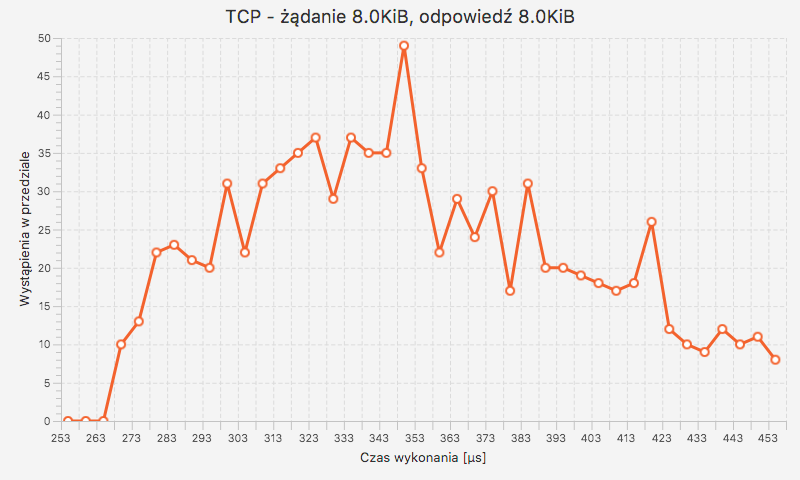
\includegraphics[scale=0.38]{img/charts/TCP_chart_8192_8192.png}
    \caption{Przykładowy wykres rozkładu czasów wykonania dla TCP}
\end{figure}

\begin{figure}[H]
    \centering
    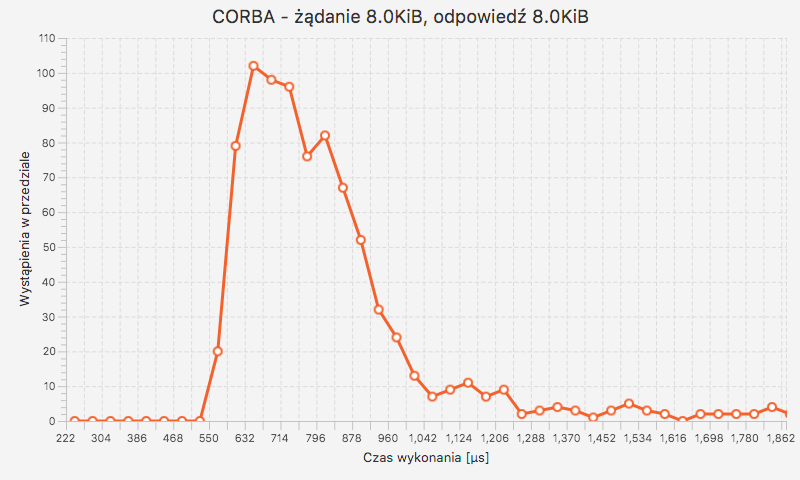
\includegraphics[scale=0.38]{img/charts/CORBA_chart_8192_8192.png}
    \caption{Przykładowy wykres rozkładu czasów wykonania dla technologii CORBA}
\end{figure}

\begin{figure}[H]
    \centering
    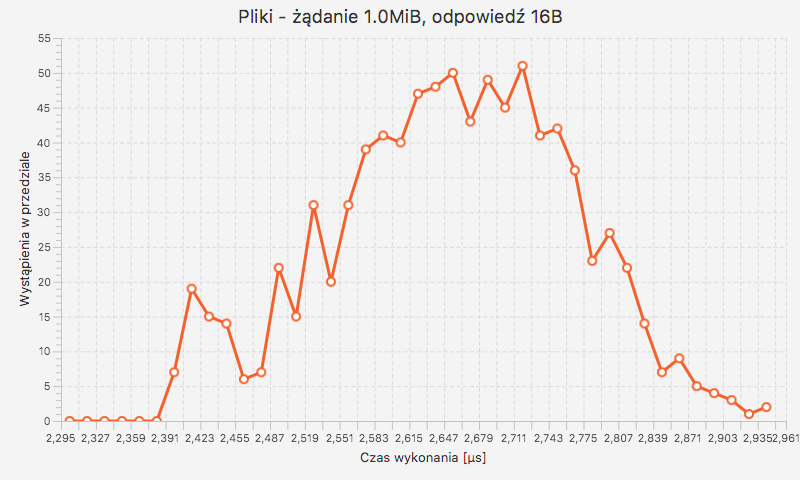
\includegraphics[scale=0.38]{img/charts/FILE_chart_1048576_16.png}
    \caption{Przykładowy wykres rozkładu czasów wykonania dla plików}
\end{figure}


\section{Porównanie wyników}

Najważniejszym zestawieniem jest porównanie czasów komunikacji dla różnych kanałów transmisji danych, przy takim samym rozmiarze przesyłanych danych. Poniżej zaprezentowane zostaną przykładowe wykresy. Zaprezentowane zostaną średnie oraz odchylenia standardowe. Wartości dla \textit{Mock} oznaczają implementację, która nie transmituje danych, tylko od razu je zwraca.


\begin{figure}[H]
\begin{tikzpicture}
\begin{axis}[
    title = {Żądanie 1KiB, odpowiedź 1KiB},
    width=15cm,
    height=8cm,
    xtick={1,...,6},
    xticklabels={
        CORBA,
        Pliki,
        JNI,
        Mock,
        REST,
        TCP
    },
    ymin=0,
    ylabel={średnia [$\mu$s]},
    nodes near coords,
    grid=major,
    ybar
]
\addplot[
    fill=blue!25,
    draw=black,
    point meta=y,
    every node near coord/.style={inner ysep=5pt},
    error bars/.cd,
    y dir=both,
    y explicit
]
table [y error=error] {
    x       y        error     label
    1   1177     1435      1
    2   2571     1151      2
    3   12         283        3
    4   6           168        4
    5   1500     176        5
    6   343       88          6
};
\end{axis}
\end{tikzpicture}
\caption{}
\label{fig:chart_1024_1024}
\end{figure}


Większość porównań dla innych rozmiarów danych jest proporcjonalna do wykresu \ref{fig:chart_1024_1024}. Pierwsze wnioski ukazują, że komunikacja przez pliki jest najwolniejsza, REST niewiele szybszy, a zdecydowanie najlepiej sprawuje się JNI.


\begin{figure}[H]
\begin{tikzpicture}
\begin{axis}[
    title = {Żądanie 16B, odpowiedź 1MiB},
    width=15cm,
    height=8cm,
    xtick={1,...,6},
    xticklabels={
        CORBA,
        Pliki,
        JNI,
        Mock,
        REST,
        TCP
    },
    ymin=0,
    ylabel={średnia [$\mu$s]},
    nodes near coords,
    grid=major,
    ybar
]
\addplot[
    fill=blue!25,
    draw=black,
    point meta=y,
    every node near coord/.style={inner ysep=5pt},
    error bars/.cd,
    y dir=both,
    y explicit
]
table [y error=error] {
    x       y        error     label
    1   5586     1553      1
    2   3854     1380      2
    3   381       317        3
    4   101       263        4
    5   13979   2194      5
    6   1976     660        6
};
\end{axis}
\end{tikzpicture}
\caption{}
\label{fig:chart_16_1048576}
\end{figure}

\begin{figure}[H]
\begin{tikzpicture}
\begin{axis}[
    title = {Żądanie 1MiB, odpowiedź 16B},
    width=15cm,
    height=8cm,
    xtick={1,...,6},
    xticklabels={
        CORBA,
        Pliki,
        JNI,
        Mock,
        REST,
        TCP
    },
    ymin=0,
    ylabel={średnia [$\mu$s]},
    nodes near coords,
    grid=major,
    ybar
]
\addplot[
    fill=blue!25,
    draw=black,
    point meta=y,
    every node near coord/.style={inner ysep=5pt},
    error bars/.cd,
    y dir=both,
    y explicit
]
table [y error=error] {
    x       y        error     label
    1   5459     1240      1
    2   2834     1233      2
    3   71         104        3
    4   3           94          4
    5   64170   9701      5
    6   1146     200        6
};
\end{axis}
\end{tikzpicture}
\caption{}
\label{fig:chart_1048576_16}
\end{figure}


Wykresy \ref{fig:chart_16_1048576} i \ref{fig:chart_1048576_16} prezentują różnicę w przypadku dużych zapytań i odpowiedzi. Należy pamiętać, że czas generowania wiadomości zwrotnej wlicza się do czasu komunikacji, więc czasy nie mogą być równe.
Dostrzec można również wielką dysproporcję w przypadku RESTa - prawdopodobnie wynika z niewydajnej implementacji biblioteki użytej po stronie serwera. 

\begin{figure}[H]
\begin{tikzpicture}
\begin{axis}[
    title = {Żądanie 16B, odpowiedź 16B},
    width=15cm,
    height=8cm,
    xtick={1,...,6},
    xticklabels={
        CORBA,
        Pliki,
        JNI,
        Mock,
        REST,
        TCP
    },
    ymin=0,
    ylabel={średnia [$\mu$s]},
    nodes near coords,
    grid=major,
    ybar
]
\addplot[
    fill=blue!25,
    draw=black,
    point meta=y,
    every node near coord/.style={inner ysep=5pt},
    error bars/.cd,
    y dir=both,
    y explicit
]
table [y error=error] {
    x       y        error     label
    1   1224     1486      1
    2   2579     1273      2
    3   6.5        144        3
    4   3.7        100        4
    5   1495     269        5
    6   338       73          6
};
\end{axis}
\end{tikzpicture}
\caption{}
\label{fig:chart_16_16}
\end{figure}

\begin{figure}[H]
\begin{tikzpicture}
\begin{axis}[
    title = {Żądanie 128MiB, odpowiedź 128MiB},
    width=15cm,
    height=8cm,
    xtick={1,...,6},
    xticklabels={
        Pliki,
        JNI,
        Mock,
        TCP
    },
    ymin=0,
    ylabel={średnia [$ms$]},
    nodes near coords,
    grid=major,
    ybar
]
\addplot[
    fill=blue!25,
    draw=black,
    point meta=y,
    every node near coord/.style={inner ysep=5pt},
    error bars/.cd,
    y dir=both,
    y explicit
]
table [y error=error] {
    x       y        error     label
    1   259.1     1.98      1
    2   97.57     1.6        2
    3   6.18       1.2        3
    4   89.86     1.6        4
};
\end{axis}
\end{tikzpicture}
\caption{}
\label{fig:chart_134217728_134217728}
\end{figure}

Narzut wynikający z samej technologii przy minimalnych rozmiarach danych (16B) jest największy dla plików (wynika z obserwatora katalogu, który wykonuje skanowanie co 2ms). Wysoki okazuje się także dla RESTa (protokół HTTP oraz serializacja do formatu JSON). Sam mechanizm, którego używa CORBA, pochłania 1ms.


JNI okazuje się najszybszą metodą przekazywania danych do aplikacji natywnych. Cechuje się też stabilnością (niskie odchylenie standardowe). Nie pozwala jednak na wywołanie zdalne, a jedynie na lokalne, synchroniczne wykonanie metody.




Implementacja testowa (bez transportu danych) zgodnie z przewidywaniami okazała się najszybsza. Udowadnia, że dla prostych metod (w tym przypadku zwykłej pętli) nie warto wykorzystywać natywnych języków i lepiej zdać się na optymalizacje wirtualnej maszyny Javy, gdyż unikniemy wtedy narzutów związanych z komunikacją.


\section{tmp}

wnioski z testów:
- wykresy

implementacja - co może jeszcze:
- rozmiar każdej z technologii (np. linie kodu, rozmiar w bajtach): CORBA omniORB około 10MB, JNI 0, TCP 0, REST, pliki
